\ifdefined\included
\else
\documentclass[a4paper,11pt,twoside]{StyleThese}
\usepackage{amsmath,amssymb, amsthm}             % AMS Math
\usepackage[T1]{fontenc}
\usepackage[utf8x]{inputenc}
\usepackage{babel}
\usepackage{datetime}

\usepackage{silence}

\WarningFilter{minitoc(hints)}{W0023}
\WarningFilter{minitoc(hints)}{W0028}
\WarningFilter{minitoc(hints)}{W0030}

\usepackage{lmodern}
\usepackage{tabularx}
%\usepackage{tabular}
\usepackage{multirow}
\usepackage{xspace}

\usepackage{subfig}
\usepackage[inline]{enumitem}

\usepackage{hhline}
\usepackage[left=1.5in,right=1.3in,top=1.1in,bottom=1.1in,includefoot,includehead,headheight=13.6pt]{geometry}
\renewcommand{\baselinestretch}{1.05}

% Table of contents for each chapter

\usepackage[nottoc, notlof, notlot]{tocbibind}
\usepackage{minitoc}
\setcounter{minitocdepth}{2}
\mtcindent=15pt
% Use \minitoc where to put a table of contents

\usepackage{aecompl}

% Glossary / list of abbreviations

\usepackage[intoc]{nomencl}
\iftoggle{ThesisInEnglish}{%
\renewcommand{\nomname}{Glossary}
}{ %
\renewcommand{\nomname}{Liste des Abréviations}
}

\usepackage{etoolbox}
\renewcommand\nomgroup[1]{%
  \item[\bfseries
  \ifstrequal{#1}{A}{Number Sets}{%
  \ifstrequal{#1}{G}{Agents Beliefs and Action Models}{%
  \ifstrequal{#1}{N}{Navigation}{%
  \ifstrequal{#1}{O}{Ontology}{%
  \ifstrequal{#1}{R}{Referring Expression Generation}{%
  \ifstrequal{#1}{Z}{Controllable and Uncontrollable Agents Task Planning}{}}}}}}%
]}

\makenomenclature



% My pdf code

\usepackage{ifpdf}

\ifpdf
  \usepackage[pdftex]{graphicx}
  \DeclareGraphicsExtensions{.jpg}
  \usepackage[pagebackref,hyperindex=true]{hyperref}
  \usepackage{tikz}
  \usetikzlibrary{arrows,shapes,calc}
\else
  \usepackage{graphicx}
  \DeclareGraphicsExtensions{.ps,.eps}
  \usepackage[dvipdfm,pagebackref,hyperindex=true]{hyperref}
\fi

\graphicspath{{.}{images/}}

%% nicer backref links. NOTE: The flag ThesisInEnglish is used to define the
% language in the back references. Read more about it in These.tex

\iftoggle{ThesisInEnglish}{%
\renewcommand*{\backref}[1]{}
\renewcommand*{\backrefalt}[4]{%
\ifcase #1 %
(Not cited.)%
\or
(Cited in page~#2.)%
\else
(Cited in pages~#2.)%
\fi}
\renewcommand*{\backrefsep}{, }
\renewcommand*{\backreftwosep}{ and~}
\renewcommand*{\backreflastsep}{ and~}
}{%
\renewcommand*{\backref}[1]{}
\renewcommand*{\backrefalt}[4]{%
\ifcase #1 %
(Non cité.)%
\or
(Cité en page~#2.)%
\else
(Cité en pages~#2.)%
\fi}
\renewcommand*{\backrefsep}{, }
\renewcommand*{\backreftwosep}{ et~}
\renewcommand*{\backreflastsep}{ et~}
}

% Links in pdf
\usepackage{color}
\definecolor{linkcol}{rgb}{0,0,0.4} 
\definecolor{citecol}{rgb}{0.5,0,0} 
\definecolor{linkcol}{rgb}{0,0,0} 
\definecolor{citecol}{rgb}{0,0,0}
% Change this to change the informations included in the pdf file

\hypersetup
{
bookmarksopen=true,
pdftitle="Endowing the robot with the abilities to control and evaluate its contribution to a human-robot joint action",
pdfauthor="Amandine MAYIMA", %auteur du document
pdfsubject="Thèse", %sujet du document
%pdftoolbar=false, %barre d'outils non visible
pdfmenubar=true, %barre de menu visible
pdfhighlight=/O, %effet d'un clic sur un lien hypertexte
colorlinks=true, %couleurs sur les liens hypertextes
pdfpagemode=None, %aucun mode de page
pdfpagelayout=SinglePage, %ouverture en simple page
pdffitwindow=true, %pages ouvertes entierement dans toute la fenetre
linkcolor=linkcol, %couleur des liens hypertextes internes
citecolor=citecol, %couleur des liens pour les citations
urlcolor=linkcol %couleur des liens pour les url
}

% definitions.
% -------------------

\setcounter{secnumdepth}{3}
\setcounter{tocdepth}{2}

% Some useful commands and shortcut for maths:  partial derivative and stuff

\newcommand{\pd}[2]{\frac{\partial #1}{\partial #2}}
\def\abs{\operatorname{abs}}
\def\argmax{\operatornamewithlimits{arg\,max}}
\def\argmin{\operatornamewithlimits{arg\,min}}
\def\diag{\operatorname{Diag}}
\newcommand{\eqRef}[1]{(\ref{#1})}

\usepackage{rotating}                    % Sideways of figures & tables
%\usepackage{bibunits}
%\usepackage[sectionbib]{chapterbib}          % Cross-reference package (Natural BiB)
%\usepackage{natbib}                  % Put References at the end of each chapter
                                         % Do not put 'sectionbib' option here.
                                         % Sectionbib option in 'natbib' will do.
\usepackage{fancyhdr}                    % Fancy Header and Footer

% \usepackage{txfonts}                     % Public Times New Roman text & math font
  
%%% Fancy Header %%%%%%%%%%%%%%%%%%%%%%%%%%%%%%%%%%%%%%%%%%%%%%%%%%%%%%%%%%%%%%%%%%
% Fancy Header Style Options

\pagestyle{fancy}                       % Sets fancy header and footer
\fancyfoot{}                            % Delete current footer settings

%\renewcommand{\chaptermark}[1]{         % Lower Case Chapter marker style
%  \markboth{\chaptername\ \thechapter.\ #1}}{}} %

%\renewcommand{\sectionmark}[1]{         % Lower case Section marker style
%  \markright{\thesection.\ #1}}         %

\fancyhead[LE,RO]{\bfseries\thepage}    % Page number (boldface) in left on even
% pages and right on odd pages
\fancyhead[RE]{\bfseries\nouppercase{\leftmark}}      % Chapter in the right on even pages
\fancyhead[LO]{\bfseries\nouppercase{\rightmark}}     % Section in the left on odd pages

\let\headruleORIG\headrule
\renewcommand{\headrule}{\color{black} \headruleORIG}
\renewcommand{\headrulewidth}{1.0pt}
\usepackage{colortbl}
\arrayrulecolor{black}

\fancypagestyle{plain}{
  \fancyhead{}
  \fancyfoot{}
  \renewcommand{\headrulewidth}{0pt}
}

%\usepackage{MyAlgorithm}
%\usepackage[noend]{MyAlgorithmic}
\usepackage{algorithm}
\usepackage[noend]{algpseudocode}
\usepackage{comment}
\usepackage[ED=MITT-InfoTel, Ets=INSA]{tlsflyleaf}
%%% Clear Header %%%%%%%%%%%%%%%%%%%%%%%%%%%%%%%%%%%%%%%%%%%%%%%%%%%%%%%%%%%%%%%%%%
% Clear Header Style on the Last Empty Odd pages
\makeatletter

\def\cleardoublepage{\clearpage\if@twoside \ifodd\c@page\else%
  \hbox{}%
  \thispagestyle{empty}%              % Empty header styles
  \newpage%
  \if@twocolumn\hbox{}\newpage\fi\fi\fi}

\newcommand*{\algrule}[1][\algorithmicindent]{%
	\makebox[#1][l]{%
		\hspace*{.2em}% <------------- This is where the rule starts from
		\vrule height .75\baselineskip depth .25\baselineskip
	}
}

%%% to have lines in algorithm, from stackexchange
\newcount\ALG@printindent@tempcnta
\def\ALG@printindent{%
	\ifnum \theALG@nested>0% is there anything to print
	\ifx\ALG@text\ALG@x@notext% is this an end group without any text?
	% do nothing
	\else
	\unskip
	% draw a rule for each indent level
	\ALG@printindent@tempcnta=1
	\loop
	\algrule[\csname ALG@ind@\the\ALG@printindent@tempcnta\endcsname]%
	\advance \ALG@printindent@tempcnta 1
	\ifnum \ALG@printindent@tempcnta<\numexpr\theALG@nested+1\relax
	\repeat
	\fi
	\fi
}
% the following line injects our new indent handling code in place of the default spacing
\patchcmd{\ALG@doentity}{\noindent\hskip\ALG@tlm}{\ALG@printindent}{}{\errmessage{failed to patch}}
\patchcmd{\ALG@doentity}{\item[]\nointerlineskip}{}{}{} % no spurious vertical space
% end vertical rule patch for algorithmicx

\makeatother
 
%%%%%%%%%%%%%%%%%%%%%%%%%%%%%%%%%%%%%%%%%%%%%%%%%%%%%%%%%%%%%%%%%%%%%%%%%%%%%%% 
% Prints your review date and 'Draft Version' (From Josullvn, CS, CMU)
\newcommand{\reviewtimetoday}[2]{\special{!userdict begin
    /bop-hook{gsave 20 710 translate 45 rotate 0.8 setgray
      /Times-Roman findfont 12 scalefont setfont 0 0   moveto (#1) show
      0 -12 moveto (#2) show grestore}def end}}
% You can turn on or off this option.
% \reviewtimetoday{\today}{Draft Version}
%%%%%%%%%%%%%%%%%%%%%%%%%%%%%%%%%%%%%%%%%%%%%%%%%%%%%%%%%%%%%%%%%%%%%%%%%%%%%%% 

\newenvironment{maxime}[1]
{
\vspace*{0cm}
\hfill
\begin{minipage}{0.5\textwidth}%
%\rule[0.5ex]{\textwidth}{0.1mm}\\%
\hrulefill $\:$ {\bf #1}\\
%\vspace*{-0.25cm}
\it 
}%
{%

\hrulefill
\vspace*{0.5cm}%
\end{minipage}
}

\let\minitocORIG\minitoc
\renewcommand{\minitoc}{\minitocORIG \vspace{1.5em}}

\usepackage{multirow}
%\usepackage{slashbox}

\newenvironment{bulletList}%
{ \begin{list}%
	{\tiny$\bullet$}%
	{\setlength{\labelwidth}{25pt}%
	 \setlength{\leftmargin}{30pt}%
	 \setlength{\itemsep}{-0.5em}}}%
{ \end{list} }

\newenvironment{inlineEnumerate}
{\begin{enumerate*} [label={(\arabic*)}] }
{\end{enumerate*}}

\theoremstyle{definition}
\newtheorem{definition}{Definition}
\renewcommand{\epsilon}{\varepsilon}

% centered page environment

\newenvironment{vcenterpage}
{\newpage\vspace*{\fill}\thispagestyle{empty}\renewcommand{\headrulewidth}{0pt}}
{\vspace*{\fill}}

\newenvironment{asl}{\ttfamily\begin{tabbing}~~~\=$\leftarrow$ \= ~~~ \=
		\kill}{\end{tabbing}}

\usepackage{tablefootnote}

\theoremstyle{plain}
\newtheorem{constraint}{Constraint}[section]

\algnewcommand\algorithmicforeach{\textbf{for each}}
\algnewcommand\algorithmicin{\textbf{in}}
\algdef{S}[FOR]{ForEach}[2]{\algorithmicforeach\ #1\ \algorithmicin\ #2\ \algorithmicdo}

\algnewcommand\algorithmicforkxor{\textbf{do fork-join-xor}}
\algnewcommand\algorithmicendforkxor{\textbf{end fork-join-xor}}
\algdef{SE}{ForkXor}{EndForkXor}{\algorithmicforkxor}{\algorithmicendforkxor}


\usepackage{listings}
\lstset{
	frame=single,
	captionpos=b,
	breaklines=true,
	basicstyle=\ttfamily,
	numberstyle=\color{black},
	tabsize=2,
	mathescape=true,
	literate=%
		{â}{{\^a}}1
}

\lstdefinestyle{inline}{
	frame=none,
	aboveskip=\smallskipamount,
	belowskip=\smallskipamount,
}

\lstdefinestyle{OwlTurtle}{
	language=C,
	tabsize=4,
	basicstyle=\scriptsize\ttfamily,
	keywordstyle=\bfseries\color{darkgray},
	morekeywords={rdf:type, rdfs:domain, rdfs:subPropertyOf, rdfs:range, :hasSubtask, :DecompositionUsedBy, rdfs:subClassOf, :hasDecomposition, owl:inverseOf, htn_actions:hasEffect, rdfs:label},
	alsoletter=:
}

\lstdefinestyle{aslDef}{
	frame=none,
%	breaklines=false,
	%xleftmargin=.1\textwidth, xrightmargin=.1\textwidth
}

\fancypagestyle{example}{%
	\fancyhead[LE]{\bfseries\thepage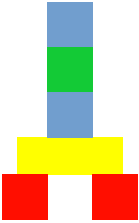
\includegraphics[scale=0.20]{figures/chapter2/task_goal.pdf}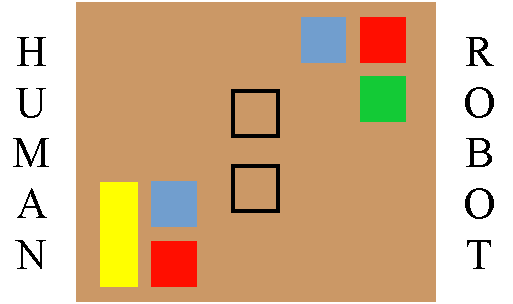
\includegraphics[scale=0.18]{figures/chapter2/task_setup_mini.pdf}}   
	\fancyhead[RO]{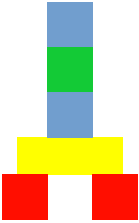
\includegraphics[scale=0.20]{figures/chapter2/task_goal.pdf}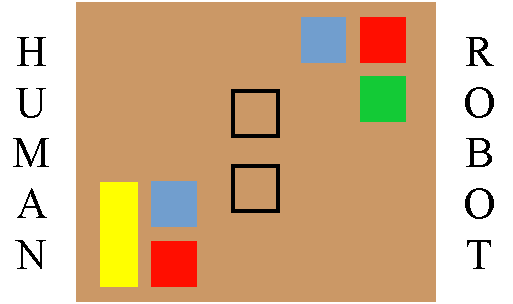
\includegraphics[scale=0.18]{figures/chapter2/task_setup_mini.pdf}\bfseries\thepage}  
	\fancyhead[RE]{\bfseries\nouppercase{\leftmark}}      % Chapter in the right on even pages
	\fancyhead[LO]{\bfseries\nouppercase{\rightmark}}     % Section in the left on odd pages
}%

\usepackage{pdfpages}
\usepackage{makecell}
\usepackage{pdflscape} 
\usepackage{mathtools}
\usepackage[section]{placeins}
\usepackage{afterpage}

%%%%%%%% my commands
\newcommand{\etal}{\textit{et al}.}
\newcommand{\ie}{\textit{i.e.}, }
\newcommand{\eg}{\textit{e.g.}, }
\newcommand{\fact}[3]{\mbox{\textit{#1}(#2, #3)}}
\newcommand{\circledtext}[1]{\raisebox{.5pt}{\textcircled{\raisebox{-.9pt} {#1}}}}
\newcommand{\sparql}{\textsc{SPARQL}}

\newcommand{\algConst}[1]{${\scriptscriptstyle #1}$}
\newcommand{\algNormTextSub}[2]{$\text{#1}_{#2}$}

\newcommand{\aslnumber}[1]{$#1$}
\newcommand{\aslstring}[1]{\textsf{#1}}
\newcommand{\aslvar}[1]{\textcolor{purple}{\textit{#1}}}
\newcommand{\asllabel}[1]{\textbf{#1}}
\newcommand{\annotation}[1]{{\footnotesize #1}}
\newcommand{\rulebody}[1]{\mbox{\hspace{.05\linewidth}}\begin{minipage}[t]{0.9\linewidth}#1.\end{minipage}}
\newcommand{\context}[1]{\begin{minipage}[t]{0.9\linewidth}#1\end{minipage}}
\newcommand{\planbody}[1]{\begin{minipage}[t]{0.9\linewidth}#1.\end{minipage}}
\newcommand{\Jason}[0]{\textbf{\textit{Jason}}}
\newcommand{\sn}{\mbox{\large\textbf{\texttt{\textasciitilde}}}}


\sloppy
\begin{document}
	\setcounter{chapter}{1} %% Numéro du chapitre précédent ;)
	\dominitoc
	\faketableofcontents
	\fi


\chapter{The ``special case'' of Human-Robot Interaction}
\minitoc
\section{Human-Robot Social Interactions}\label{chap1:sec:soc_inter}

Now that we have seen how social interactions look like when happening between humans, we are going to see the different ways the human-robot interaction field divided and categorized interactions. It is possible to define an interaction according to its length as we will show in Section~\ref{chap1:subsec:inter_lengths}. Then, inside the interaction, what are the different temporal phases? We will see it in Section~\ref{chap1:subsec:inter_div}. Next, in Section~\ref{chap1:subsec:inter_hier}, we will take an interest in a different way to segment interactions: with hierarchical levels. Finally, some authors proposed some interaction patterns, we will present a few in Section~\ref{chap1:subsec:inter_patt}.

\subsection{Interaction lengths}\label{chap1:subsec:inter_lengths}
\paragraph{Short-term Interactions}
Zheng \etal{} defined a \emph{short-term interaction}~\cite{zheng_2013_designing} based on the Unified Theories of Cognition of Newell~\cite{newell_1994_unified}. A short-term interaction corresponds to the ``cognitive band'' of cognition, during which they focus on individual utterances and speech acts for interactions that last for tens of seconds. They left aside longer-term interactions that can be in the ``rational band'' (minutes to hours) or the ``social band'' (days to months).
Gaschler \etal{} deployed a bartender robot and defined a short-term interaction as being a customer ordering a drink – from the attention request towards the bartender to the closing of interaction by payment and exchange of polite phrases~\cite{gaschler_2012_modelling}.
Iocchi \etal{} used the \emph{short-term} to refer to short interactions and that are focused on only one particular communicative objective, avoiding long and complex interactions~\cite{iocchi_2015_personalized}.
Sanelli \etal{} gave three characteristics to a short-term human-robot interaction: (1) users are not familiar with the robot (2) each interaction happens with a different user (3) interaction is short in time. Then, the robot has not memory of past interactions~\cite{sanelli_2017_short}.

\paragraph{Long-term Interactions}
A survey~\cite{leite_2013_social} has been done by Leite \etal{} about long-term human-robot interactions, where long-term means, most of the time, several interactions between the same human and robot. They defined four contexts for which social robots\footnote{actually, some of the robots featured in the survey are not social robots such as a Roomba or the Personal Exploration Rover (PER)} for long-term interaction have been designed: health care and therapy, education, work environment and public spaces, and people's homes. 

For example, Kanda \etal{} performed a field trial at an elementary school in Japan for two months~\cite{kanda_2007_two}. The children were able to interact with the robot for 32 days in total, during 30 minutes after lunch. The robot could switch between one hundred pre-defined behaviors (\eg hugging, shaking hand or singing) but not all of them were available during the first interactions with a human. Indeed, they had integrated a pseudo-development mechanism, \ie the more a child interacts with the robot, the more different behaviours the robot displays to that child. Also, the robot confided personal-themed matters to children who have often interacted with it (\eg ``I don't like the cold''). These abilities allowed the robot to maintain the children's interest even after the first week whereas in a first experiment where the robot's behavior was the same all along the two months, most children stopped to interact with the robot from the second week. 

In their discussion, Kanda \etal{} raised an interesting question: `` How Long Should \textquoteleft Long-Term\textquoteright{} Be?'' They found out that some authors consider that two months is a long-term interaction. They also pointed that some Human-Computer Interaction studies on long-term interaction last five weeks. In their survey, Leite \etal{} gave their point of view, which seems well-thought. They argued that it is more important to look at the number of interaction sessions and the length of these sessions (a five minutes-interaction is different from a one hour-interaction). For them, an interaction can be considered as long-term when the user becomes familiarized with the robot to a point that their perception of such robot is not biased by the novelty effect anymore. This definition raises another question: when does user’s familiarization with the robot become stable? But we will not discuss it here.

\subsection{Interactions divided in phases}\label{chap1:subsec:inter_div}
Among works on short-term or long-term interactions, some authors divided interactions in phases which have sometimes similarities with the phases of social interactions described in Section~\ref{chap1:sec:soc_int}.

Gockley \etal{} divided an interaction in three phases: greeting, core of the interaction and departure~\cite{gockley_2005_designing}. In the greeting phase, Valerie, the robot receptionist, greets people who might be interested in engaging in conversation. Thus, people are classified into ``attentional'' states:
\begin{bulletList}
	\item present (people a bit far and moving): Valerie doesn’t pay attention to them
	\item attending (people closer): Valerie greets them
	\item engages (people next to the desk but on the side): Valerie acknowledges their presence but does not expect input from them
	\item interacting (people in front of the keyboard): Valerie prompts them for input if they are not typing.
\end{bulletList}
In the core of interaction, either Valerie can tell her (fictive) story or chat. Her story is subjective and evolve over time. It is about her social life, her lounge singing career, her therapy business, and her job as a receptionist. Furthermore, Valerie has a chatbot system which is very simple. Finally, inputs from visitors are from a keyboard, for easier control and reliability. Finally, at departure, when a person leaves the ``interacting'' region, Valerie signals the end of the interaction by saying ``goodbye''. 

Kidd and Breazeal presented robot which is a weigh loss coach~\cite{kidd_2008_robots}. They introduced here the notion of states of relationship. They are three: initial (for the first few days of interaction), normal, repair. According to the state of relationship, the robot answers/questions/speech will not be the same. Kasap and Magnenat-Thalmann designed their system so, to each user, corresponds an interaction session~\cite{kasap_2012_building}. Each session is composed of four dialogue phases: welcome, warm up, teach and farewell. The system has a memory of users and past interactions. In the memory, is recorded the context (initial state and goal), contents (events) and the outcome (goal succeeded or not). A bit similar to the relationship state defined by Kidd and Breazeal~\cite{kidd_2008_robots}, they defined a notion that they call relationship level. It is computed based of the emotional interactions from the episodic memory associated to a user. It influences the mood level of the robot and then the facial expression and the speech.

In the work around the bartender robot~\cite{gaschler_2012_modelling}, they divided the interaction in three phases (or states) but from two different viewpoints, the of the customer and the one of the bartender. From the customer viewpoints, the phases are: (1) attention request towards bartender (2) ordering of one or more beverages, and (3) closing of interaction by payment and exchange of polite phrases. Then, in reaction of each phases, there are the ones from the bartender viewpoint: (1) acknowledging the attention request, (2) serving the ordered drink, and (3) asking for payment.
They left open the possibility to have sub-phases inside phases.

We can also find, in Lee \etal{}' work~\cite{lee_2012_personalization}, the notion of structure of interaction: interactions start with the vendor identifying the customer, greeting and engaging in small talk with the customer, engaging in the snack transaction, and then enacting social leave-taking.

\subsection{Hierarchical interactions}\label{chap1:subsec:inter_hier}
Not only, interactions can be divided in phases but also in levels. For example, Dautenhahn and colleagues~\cite{dautenhahn_2002_embodied, ogden_2001_interactional} defined two levels of approach for interactions, a global one and a local one. The \emph{global level approach} defines a unit of interaction as being relatively large (long sequences of interaction or large units of interaction), such as the script for a greeting as described by Kendon in~\cite{kendon_1990_conducting}. At this level, an interaction may be seen as a unit similar to a schema or script, in the computer/cognitive science senses of these terms. They named this level of interaction a ``Global Interactional Unit (GIU)''. Furthermore, a GIU can be divided in phases, each of which has associated behaviors. Behaviors have meaning and their meaning depends on the phase in which they occur, the context (\eg a ‘wave hello’ vs. a ‘wave goodbye’). Their \emph{local level approach} is a much smaller unit, often as simple as an action and a response to that action. They claimed that this view of interaction has the advantage of greater flexibility and robustness compared to the globally structured view. Flexibility is a result of the possibility of specifying acts that may occur in many global interactional structures. But, as contextual details are ignored, the ability to assign a specific meaning to an action is lost.

In his thesis, Kuo insists about this flexibility and the re-usability~\cite{kuo_2012_designing}. A lower level of design is more appropriate for reuse. For him, a unit of interaction corresponds to an ``interaction cue'' (or social cue) that a robot can perceive and act upon or express in an interaction. These cues can be verbal, non-verbal, or a combination of both (multi-modal interaction). A complete episode of interaction should be constructed through composition of interaction cues with some common patterns repeated over the course of the interaction (\eg awareness of human presence).

\subsection{Patterns of Interaction}\label{chap1:subsec:inter_patt}
Before talking about design patterns or interaction patterns, Goffman argued that human interactions follow a specific ``order'' and characterized a number of patterns in which people interact, such as how greetings unfold and how people leave an interaction~\cite{goffman_1983_interaction}.

Kahn \etal{} introduced design patterns~\cite{kahn_2008_design}, that they will later called interaction patterns in~\cite{kahn_2010_validating}, inspired from computer science. They proposed rules to follow using them and eight patterns. The two main ideas to retain is that a sequence of patterns has to be well ordered and that patterns can be hierarchical. 
The 8 patterns: 
\begin{bulletList}
	\item The initial introduction: largely scripted, conventionally-established verbal and behavioral repertoire to recognize the other, inquire politely about the other, engage in some physical acknowledgment (\eg handshake)
	\item Didactic communication: one-way communication of information 
	\item In motion together: walk together
	\item Personal interests and history: sharing of personal interests and history with others
	\item Recovering from mistakes: creates the potential for both parties to maintain a social affiliation following the mistake
	\item Reciprocal turn-taking in game contextual: taking turns with one another when playing games
	\item Physical intimacy: to engage in holding or touching or embracing
	\item Claiming unfair treatment or wrongful harms: allows to make claim to its moral standing
\end{bulletList}


Following the same idea and going further, Sauppé and Mutlu introduced the interaction blocks~\cite{sauppe_2014_design}. Compared to Kahn’s work, they created a pattern language and a tool/environment to design human-robot interaction. To conceive their patterns, they collected and analyzed data from 5 kinds of interaction scenarios: Conversation, Collaboration, Instruction, Interview and Storytelling.
Then, they identified common interaction structures, which served as ``design interaction patterns'':
\begin{bulletList}
	\item Introductory monologue: A short introduction can be used to introduce other participants to a scenario by giving an overview of the remainder of the interaction or it can be a greeting for example.
	\item Question and Answer: A question is a sentence meant to elicit information from other participants. An answer is the response to a question that aims to satisfy the questioning participant’s curiosity.
	\item Generic Comment and Personal Comment: A comment is a short statement offering the speaker’s opinion. Comments are either generic (\eg, ``Wow'') or personal (\eg, ``I tried that and didn’t like it'').
	\item Monologue and Generic Comment: A monologue is a longer form of speech during which no response is expected.(\eg telling of a story). Although monologues expect no response, listeners may occasionally offer unsolicited commentary.
	\item Instruction and Action: An instruction is a command offered by one participant to direct the actions of another participant. The proper response to this instruction is often an action, although the action might follow the instruction with a delay depending on whether it is an appropriate time to perform that action
	\item Finished Comment: Upon the completion of the goals of the scenario, one or more of the participants will note that the scenario is completed by offering a finished comment.
	\item Wait: One pattern implicit in all scenarios involving two or more participants is the wait pattern.
\end{bulletList}
Finally, they designed a software to easily implement those patterns in a robot.

In his thesis, Kuo criticizes Kahn’s work~\cite{kuo_2012_designing}. He says that these patterns involve sequences of interaction cues and should be decomposed to a lower level for detailed design and reuse. He proposed his own patterns:
\begin{bulletList}
	\item Human presence detection: detect when there is a person who might be interested in
	\item Showing interest for interaction: express the robot’s awareness of a user’s presence around it and its interest and willingness to interact
	\item User’s attention on the robot: Know when a user is paying attention to the robot in an interaction and its information on its screen
	\item User identification by face: Provides the fundamental block for personal service and social interaction by recognizing the human counterpart in an interaction
\end{bulletList}
He checked the validity of his patterns with the analysis of Problem statement, Context of Use, Interaction Modality, Combination with Other Patterns, Technical Performance and Limitations, User Feedback and User’s Perception, Resulting Interactive Behavior.

Finally, Peltason and Wrede also based their work on design patterns from computer science, specifically applied to dialogue here~\cite{peltason_2010_pamini}. To name a few of them: Simple action request, Interaction opening, Interaction closing, Clarification. During interaction, the registered patterns are employed in a flexible way by admitting that patterns can be interrupted by other patterns and possibly resumed later which leads to interleaving patterns. By default, simpler patterns are permitted to be nested within temporally extended patterns.




\section{Human-Robot Interaction and Joint Action}\label{chap1:sec:hri_ja}
The study of human-human joint action is important to understand how to make robots better companions and partners for humans. However, it does not mean that they should imitate humans, as they are machines, they have their own abilities and have to develop their own strategies~\cite{bradshaw_2017_human} (\eg displaying an arrow on the floor while navigating~\cite{chadalavada_2015_mind, coovert_2014_spatial}).

In the context of the JointAction4HRI project, a non-exhaustive review of existing robotic systems integrating but also recognizing in humans joint action mechanisms has been done, focusing on joint attention, communication to facilitate coordination, repairs strategies and commitments.

\subsection{Joint Attention in HRI}
Joint attention is essential to joint action (see Section~\ref{chap1:subsubsec:joint_att}). Some authors showed that a robot initiating (\ie triggering the attention focus of the partner on the object of interest)~\cite{imai_2003_physical}, responding to (\ie gaze following of the partner's gaze or gesture)~\cite{yu_2010_investigating}, and ensuring joint attention (\ie monitoring of the other's attention)~\cite{huang_2010_joint} improves the task performance and is perceived as more natural. Thus, human pointing gesture recognition as been investigated such as in~\cite{nickel_2007_visual} or eye-gaze signaling(\eg \cite{staudte_2009_visual} or see review~\cite{admoni_2017_social}).

\subsection{Communication to Facilitate Coordination in HRI}

As seen in Section~\ref{chap1:subsec:comm}, communication is important for joint action. It is useful to negotiate, guide, question or realign the beliefs between agents as divergences might occur~\cite{cohen_1991_teamwork}. Here, we will see how robots can do to communicate and understand communications about: (1)  their internal state or the human partner's one, and (2) intentions.

\paragraph{Internal state communication -- Expressions}
It is not always obvious for the human to know what the robot is ``thinking'', \ie to know in what state is the robot. The robot also needs to be able to recognize human internal states. Roboticists developed different ways to do so. We found that robot communicating their internal state using lights, dialogue, gestures/moves or facial expressions has been developed. Some of them are also able to analyze human face or voice to detect their emotion or expression. Kim and Kwon designed a robot using all these features to generate expressions according to its knowledge about the task execution state~\cite{kim_2010_computational}. Expressions are generated based on as set of criteria. For example, when the robot computes that it is in an unexpected state, it generates surprise. Moreover, they endowed the robot the ability to discriminate between the human partner's happiness, sadness and anger. In the same spirit, we can find a robot recognizing and generating expressions through voice, in relation to the task state and goal~\cite{scheutz_2006_utility}. Finally, we have to mention the work of Breazeal which investigated a lot display of emotions/expressions in human-robot interaction. We can distinguish two types of communication: (1) a robot, which as a caregiver, has a motivation system in order to regulate the interaction intensity of its caregiver by expressing eight emotions with facial expressions~\cite{breazeal_1998_motivational, breazeal_2004_function}, (2) a robot has the ability to recognize four communication intents (approval, attentional bid, prohibition, soothing) and to react to them through speech~\cite{breazeal_2002_regulation, breazeal_2003_emotion}.

\paragraph{Communication of intentions} As explained in Section~\ref{chap1:subsubsec:coord_smooth}, coordination smoothers facilitate the prediction and legibility of a partner's action. Investigation about how the robot could communicate its intention during navigation has been done. Some authors chose to have the robot communicating its intention using lights~\cite{szafir_2015_communicating}, comparing this method with a communication using the head orientation and finding it better~\cite{may_2015_show}. Others worked on make the robot navigation legible, improving its predictability by the human~\cite{dragan_2013_legibility, alami_2006_toward}. A last method to communication navigation intention is by projecting arrows on the floor as well as a map~\cite{chadalavada_2015_mind, coovert_2014_spatial}.  Not only robot navigation should be legible but also its gestures, when handing over an object to the human~\cite{sisbot_2012_human}, or opening a door~\cite{takayama_2011_expressing} for example. Finally, a lot of works can be found on human gestures recognition so the robot could prediction human's action intentions (\eg\cite{barros_2017_dynamic, chang_2018_effects}).

\subsection{Theory of Mind in HRI}\label{chap1:subsec:tom_hri}
\acrfull{tom} is related to joint action as shown in Section~\ref{chap1:subsec:tom}. One of the first work to bind robotics and \acrshort{tom} is Scassellati~\cite{scassellati_2002_theory}. He proposed a model of a \acrshort{tom} implementation for a robot, inspired by two models from psychology: Leslie’s Model of Theory of Mind~\cite{leslie_1984_spatiotemporal} and Baron-Cohen’s Model of Theory of Mind~\cite{baron-cohen_1995_mindblindness}. His model focused on two abilities: to make the distinction between animate and inanimate visual stimuli (following Leslie's perceptual world division into animate and inanimate spheres), and to identify gaze direction (enabling the shared attention mechanism as emphasized by Baron-Cohen). 

Over the years, others tried to tackle this issue, especially focusing on perspective-taking abilities. For example, Hiatt and colleagues designed and implemented a model simulating a human with the ability to deal with false beliefs~\cite{hiatt_2010_cognitive}. They demonstrated it with the Sally--Anne test presented in Section~\ref{chap1:subsec:tom}. Milliez \etal{} endowed a robot with the ability to pass the Sally--Anne test, constructing a semantic representation of the world based on its estimation of the human's point of view~\cite{milliez_2014_framework}.

Perspective-taking abilities have been used in robotics for several purposes. Berlin \etal{} presented a simulated robot able to take the visual perspective of a human teacher (the virtual camera) and showed how this ability could be used for learning in human-robot interaction~\cite{berlin_2006_perspective}. Hiatt \etal{} presented a humanoid robot reasoning on possible beliefs the human partner could have endowing the robot with the ability to deal with uncertainty about the estimation of the human's beliefs~\cite{hiatt_2011_accommodating}. In another work, perspective-taking allows the robot to solve ambiguous references to an object~\cite{ros_2010_solving}. Others make use of perspective-taking to improve human action recognition~\cite{johnson_2005_perceptual}. Endowing a robot with a perspective-taking ability can also serve to support the implementation of an autobiographical memory (a meaningful stored knowledge acquired during interactions)~\cite{pointeau_2017_role}. Finally, it can also be a way to help the robot to elaborate plans, adding communication actions to solve divergent beliefs~\cite{warnier_2012_robot}, to explain plans to the human with a level of details depending on their knowledge~\cite{milliez_2016_using} or to manage shared plans execution~\cite{devin_2016_implemented}.

\subsection{Failures in HRI}
Honig and Oron-Gilad studied the different types of failures that could happen during a human-robot interaction and proposed a classification of these~\cite{honig_2018_understanding} based on a meticulous review, illustrated with Figure~\ref{chap1:fig:err_hri}.

\begin{figure}[!ht]
	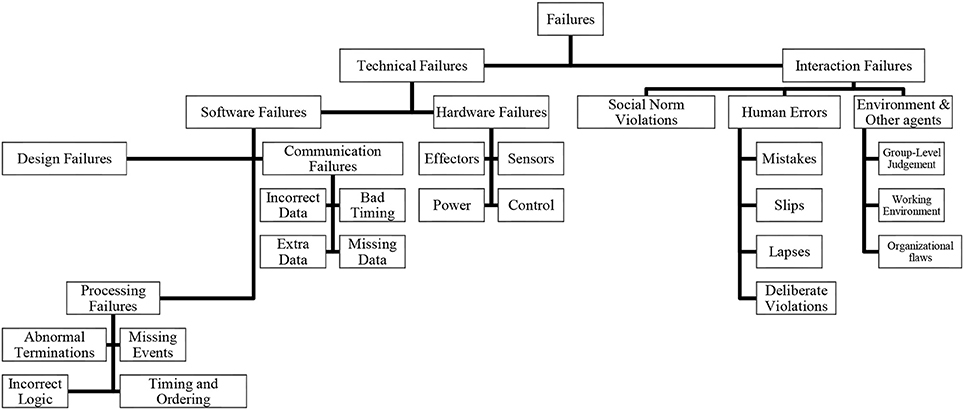
\includegraphics[width=\linewidth]{figures/chapter1/failures_hri.jpg}
	\caption{Classification of failures in HRI, realized by Honig and Oron-Gilad~\cite{honig_2018_understanding}.}
	\label{chap1:fig:err_hri}
\end{figure}

\subsubsection{Communicating about Failures}
When something unexpected happens during the interaction, either because of a human failure, a robot failure or an external event, robots might need to communicate about it. We saw three most common ways to communicate about a failure: facial expressions and speech. We can notice a less common way proposed by Kwon \etal{} which developed a robot communicating about its incapability to execute a manipulation tasks thanks to the execution of an ``attempt motion'', expressing what it cannot do and why to its human partner (\eg lifting its elbow to communicate that it is trying to lift the cup, but the cup is too heavy for it)~\cite{kwon_2018_expressing}. 

\paragraph{Facial expressions} Breazeal and colleagues investigated the expression of the robot's confusion through facial expressions. For example, in~\cite{breazeal_2002_regulation, breazeal_2003_emotion} humans take into account the robot expressive feedback to assess when the robot ``understand'' them. If the wrong expression appeared, they often speak in an exaggerated way to correct the ``misunderstanding''. Hamacher \etal{} developed a robot  displaying a facial expression after having dropped an egg when preparing an omelet with a human~\cite {hamacher_2016_believing}. Reyes \etal{} proposed a robot displaying a negative facial expression when an error occurs~\cite{reyes_2015_positive}. In work by Silva \etal, the robot decision-making and error detection/handling processes are influenced by the perceived human emotions and the robot can display facial expressions when the human persists in a error~\cite{silva_2016_combining}.

\paragraph{Speech} Most of the time, when speech is involved, it is not only to communicate about the failure but also to initiate a repair strategy. 

\subsubsection{Robot Repair Strategies}
To communicate about a failure is not enough to be able to continue the task or the interaction. A collaborative robot needs repair strategies. Some authors proposed simple strategies while some others developed more complex ones. In~\cite{li_2006_computational}, when the robot detects a failure in its understanding of the human utterance and gesture, it triggers its repair mechanism that leads the robot to ask questions to the human in order to help it disambiguate the utterance/gesture. In~\cite{morales_2019_interaction}, there were two possibilities when a failure happened: the human had an ``assistance opportunity'' (\ie failure case that caused no risk to person or property) before the failure occurrence or not. People were more willing to help the robot in case of failure with an assistance opportunity. Knepper \etal{} proposed a robot, when encountering a failure, able to request help from a human -- which might not be aware of the context. After receiving help, it resumes its autonomous task execution~\cite{knepper_2015_recovering}. Lee \etal{} compared three recovering strategies after a robot failure (but based on videos and not a real robot) to see which one was preferred by the humans: (1) apology (\ie robot apologies for service failure), (2) compensation (\ie robot provides compensation, such as an exchange, a refund, or a discount coupon), (3) option (\ie robot provides human with alternative actions to achieve their goals)~\cite{lee_2010_gracefully}. All strategies had a positive effect (even if not the same). Spexard \etal{} developed three repair strategies according to the type of failure for their robot: (1) when the robot encounters an internal issue, it informs the human about the break-down and asking them a reboot or to contact a technician, (2) it can generate appropriate speech related to error messages from its sensor, \eg the robot informs the human of the reason why it can not move and asks them for help, and (3) the robot asks for a reset if it thinks that the information it has about a human does not seem to be right~\cite{spexard_2008_oops}. Mutlu \etal{} performed a user study to compare three repair strategies in a task where the robot gives instructions to the human in an assembly task~\cite{mutlu_2013_coordination}. The strategies are: (1) ``no repair'' (\ie the robot detects an error but waits without answering to the human's questions), (2) ``simple repair'' (\ie the robot answers by yes or no to the human yes/no questions, for other questions it repeats the instruction), and (3) ``humanlike-repair'' (\ie the robot gives the appropriate information to human, triggered either by a human request, or failure or hesitancy detection). The last strategy was the preferred one by the participants.

\ifdefined\included
\else
\bibliographystyle{acm}
\bibliography{These}
\end{document}
\fi
